\documentclass[10pt]{article}
\IfFileExists{neurips_2026.sty}
  {\usepackage[preprint]{neurips_2026}}
  {\usepackage[margin=1in]{geometry}}
\usepackage{amsmath,amssymb,booktabs,graphicx,hyperref,microtype}
\usepackage[numbers]{natbib}
\usepackage{xcolor}
\newcommand{\method}{Clock-Conditioned RFE}
\title{\method{} under Controlled Gridworld Drift:\\A Reproducible Negative-Result Study}
\author{Anonymous}
\date{}

\begin{document}
\maketitle

\begin{abstract}
Reward-free exploration is usually studied in stationary Markov decision
processes.  We audit a small drifting-gridworld implementation and evaluate a
modest alternative: forward-dynamics representations conditioned on an
observable normalized clock.  The corrected implementation uses a global drift
clock across episode resets, reachable-state coverage, aligned pre/post
evaluation, deterministic seeds, and raw per-episode outputs.  Across ten
seeds, three drift types, and three feasible ablations, the conditioned
representation does not improve post-drift success.  Most methods fail on goal
and wall drift; on transition-noise drift, fixed/count obtains 0.335 mean
success versus 0.180 for time/count, with wide bounded confidence intervals.
These results are diagnostic rather than evidence of a new state-of-the-art
method.
\end{abstract}

\section{Introduction}
Reward-free exploration (RFE) separates reward-agnostic data collection from
later task learning \citep{jin2020rewardfree}.  Nonstationarity complicates this
separation because a representation learned from early transitions may cease to
describe later dynamics.  This study asks a deliberately narrow question:
does giving a forward model an observable clock help in a small controlled
gridworld?  The answer in our current experiment is no.

Our contribution is primarily methodological: we provide an auditable
implementation and expose a negative result.  We do not claim a faithful
implementation of UCRL-RFE, drift detection, minimax optimality, or novelty over
general contextual representation learning.  The explorer is a local
count-bonus heuristic.  The clock is available at training and test time, but
the method never receives the drift boundary, active map, goal, or a
``drift-applied'' bit.

\section{Related Work}
RFE seeks exploration policies or datasets useful for rewards revealed later
\citep{jin2020rewardfree}.  Optimism and confidence sets underpin classical
tabular methods such as UCRL2 \citep{jaksch2010near}; our implementation omits
their planning step and therefore avoids that name.  Nonstationary RL studies
changing rewards or transition kernels, often under variation budgets
\citep{cheung2020nonstationary}.  Deep Q-learning provides our downstream
learner \citep{mnih2015human}, while standard RL definitions follow
\citet{sutton2018reinforcement}.  Our experiment is smaller in scope than these
theoretical and large-scale empirical lines.

\section{Setting}
Let $\mathcal{M}_t=(\mathcal{S},\mathcal{A},P_t,r_t,H)$ be a finite-horizon,
time-indexed MDP.  At global transition $t$, the environment applies
$P_t(\cdot\mid s,a)$ and $r_t(s,a,s')$.  Sudden drift at $\tau$ means
$(P_t,r_t)=(P^-,r^-)$ for $t<\tau$ and $(P^+,r^+)$ for $t\geq\tau$.
The global clock does not reset at episode boundaries.

The state is the integer agent coordinate on a $6\times6$ grid and there are
four actions.  Goal drift changes $r_t$ by moving the terminal goal;
transition-noise drift changes $P_t$ by randomizing actions; wall drift changes
reachable transitions.  Coverage is
\[
 C(V;\mathcal{R})=\frac{|V\cap\mathcal{R}|}{|\mathcal{R}|},
\]
where $\mathcal{R}$ is the union of cells reachable from the start in the
configurations encountered during collection.  This excludes unreachable
cells from the denominator.

\section{Method}
\paragraph{Collection.}
The count collector chooses an action maximizing a decreasing state-action
count bonus, breaking ties with a seeded generator.  The random baseline draws
uniform actions.  Neither observes rewards.  This is not UCRL-RFE because it
does not solve an optimistic MDP.

\paragraph{Representations.}
The fixed encoder is an MLP $f_\theta(s)$ trained on the complete transition
stream.  The count-collected fixed and time-conditioned models receive
identical ordered records; their sole representation-level difference is
whether the clock is consumed.
The conditioned encoder uses
\[
\begin{aligned}
z_t&=f_\theta\!\left([s_t;g_\psi(c_t)]\right),\\
c_t&=\min(1,t/T),
\end{aligned}
\]
where $g_\psi$ is a learned clock embedding.  A predictor minimizes
$\|\hat{s}_{t+1}(z_t,a_t)-s_{t+1}\|_2^2$.  Temporal metadata is passed in every
conditioned training batch.  The encoders are frozen during downstream DQN
training.  Thus clock conditioning is tested as a representation ablation,
not as online representation adaptation.

\paragraph{Procedure (pseudocode).}
\begin{enumerate}
  \item Seed Python, NumPy, PyTorch, environment, collector, replay sampling,
  and action selection.
  \item Collect $(s_t,a_t,s_{t+1},c_t,c_{t+1})$ without reward.
  \item Train both encoders on exactly the same records; provide $c_t$ only to
  the conditioned encoder.
  \item Freeze the encoder and train DQN while environment and encoder share
  the same global clock.
  \item Evaluate each episode on the same task layout used for downstream
  training at a controlled pre- or post-drift clock; report bounded 95\%
  percentile cluster-bootstrap intervals over independent seed means.
\end{enumerate}

\section{Experiments}
\paragraph{Design.}
We use seeds 0--9, 4,000 reward-free transitions, eight representation epochs,
4,000 DQN transitions, drift at transition 2,000, 20 evaluation episodes per
phase, and a 60-step cap.  Methods are fixed/count, time/count, and
fixed/random.  Drift strength is 0.6 and there are two walls.  Hyperparameters
were selected for feasible local execution.  The 4,000-step downstream budget
was the largest member of a predeclared diagnostic, not selected because it
gave the best outcome.

\paragraph{Results.}
Table~\ref{tab:results} and Figure~\ref{fig:results} are generated directly
from the saved CSV.  Reported intervals are bounded percentile intervals from
20,000 bootstrap resamples of the ten independent seed-level means.  Episodes
within a seed are not treated as independent replicates.  The table displays
means for readability.

\begin{table}[t]
\centering
\caption{Mean success rate across ten seeds.}
\label{tab:results}
\begin{tabular}{llrr}
\toprule
Drift & Method & Pre success & Post success \\
\midrule
goal shift & fixed count & 0.00 & 0.00 \\
goal shift & time count & 0.00 & 0.00 \\
goal shift & fixed random & 0.00 & 0.00 \\
transition noise & fixed count & 0.10 & 0.33 \\
transition noise & time count & 0.00 & 0.18 \\
transition noise & fixed random & 0.00 & 0.20 \\
wall change & fixed count & 0.00 & 0.00 \\
wall change & time count & 0.00 & 0.00 \\
wall change & fixed random & 0.00 & 0.00 \\
\bottomrule
\end{tabular}

\end{table}

\begin{figure}[t]
\centering
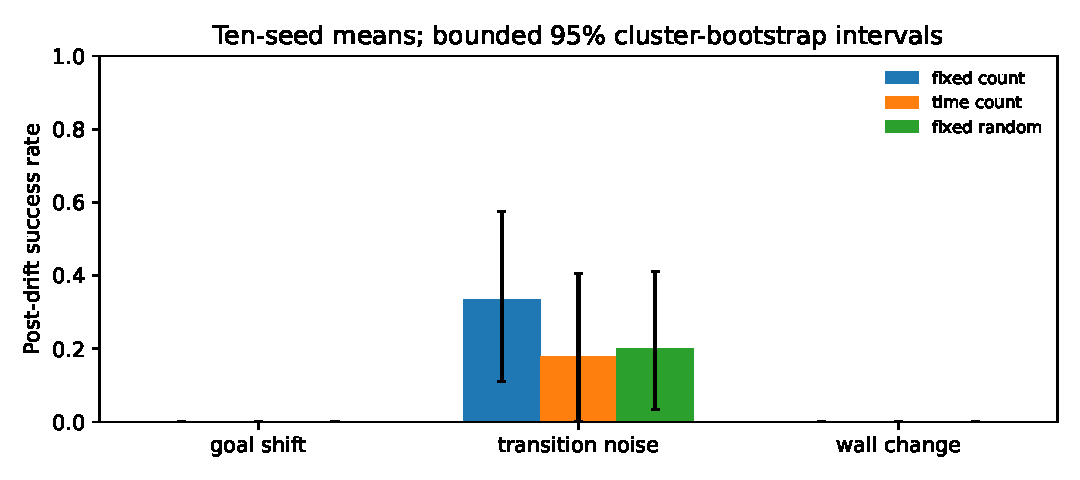
\includegraphics[width=\linewidth]{figures/post_drift_success.pdf}
\caption{Post-drift success. Error bars are bounded 95\% percentile
cluster-bootstrap intervals across ten seed-level means.}
\label{fig:results}
\end{figure}

Goal drift yields zero success for all methods in both controlled phases.
For transition-noise drift, post-drift means (95\% intervals) are 0.335
([0.110, 0.575]) for fixed/count, 0.180 ([0.000, 0.405]) for time/count, and
0.200 ([0.035, 0.410]) for fixed/random.  Under wall drift, all means are zero.
These data do not support an advantage for clock conditioning or random versus
count collection.

\begin{table}[t]
\centering
\caption{Mean reachable-state coverage during reward-free collection.}
\label{tab:coverage}
\begin{tabular}{lrr}
\toprule
Drift & Count & Random \\
\midrule
goal shift & 1.000 & 1.000 \\
transition noise & 1.000 & 1.000 \\
wall change & 1.000 & 1.000 \\
\bottomrule
\end{tabular}

\end{table}

Coverage is nearly saturated (Table~\ref{tab:coverage}), so it does not explain
downstream differences at this budget.  High coordinate coverage also need not
imply balanced transition coverage or a useful frozen representation.

\paragraph{Budget and semantic diagnostic.}
The original evaluation generated a new random goal/map while exposing only
agent coordinates, an unidentifiable task-generalization problem.  We corrected
evaluation to reuse each training task's configuration while retaining fresh
stochastic rollouts.  A predeclared goal-drift check used seeds 0--2 and
500/1,500/4,000 DQN steps.  Success was non-monotonic: fixed/count remained
zero; time/count pre/post means were 0.33/0.33, 0/0, and 0/0.33 respectively.
Thus the semantic flaw was real, but merely increasing this small sparse-reward
budget did not reliably repair DQN training.

\section{Limitations}
This is a small synthetic study with ten seeds, sparse terminal reward, one
drift strength, a 4,000-step DQN budget, and no hyperparameter sweep.  The normalized
clock assumes time is observable and can correlate with drift; this is weaker
than oracle access to the drift state but stronger than time-unaware learning.
The agent is not told $\tau$, yet a sufficiently expressive model could infer
regular timing from data.  Percentile cluster bootstrap is bounded and respects
seed clustering, but only ten clusters remain insufficient for precise tails;
all-zero samples yield degenerate intervals.  The budget check indicates
sparse-reward instability, so zero success is not evidence of impossibility.
We test no
faithful model-based optimistic RFE algorithm and make no general claim about
RFE under drift.

\section{New Experimental Direction}
Motivated by the negative clock result and the unstable DQN diagnostic, the
artifact now includes a separate, predeclared protocol for future experiments.
It estimates a categorical forward model online and applies a deterministic
two-window change test to its pre-update prediction residuals.  Alarms create
inferred regime identifiers; this detector receives transitions only, not the
global clock, drift boundary, active map, goal, or an oracle drift bit.  We
make no theorem or optimality claim for this heuristic.

The protocol compares a pooled stationary transition model, an
inferred-regime-conditioned model, and an explicitly labelled
oracle-regime upper bound.  All three receive the same ordered transition data
and use matched maximum-likelihood estimation and value iteration.  The
tabular planner is required to solve stationary grids, separating failures of
transition representation from sparse-reward DQN optimization.  Predeclared
outputs include detection delay, false alarms, post-drift recovery versus
additional samples, state-action and transition coverage, regime assignment
accuracy where schedule labels exist, and seed-level uncertainty.  Sudden,
gradual, and periodic schedules, multiple geometries and strengths, resumable
unit checkpoints, and quick/pilot/full CPU profiles are implemented.

This section specifies a direction and protocol only.  It does not replace or
reinterpret the measured clock-conditioned results above; any new numerical
claims must be generated from the new raw output directory.

\section{Reproducibility}
The canonical entry point is \texttt{run.py}; the package
\texttt{rfe\_drift/} contains the environment, collectors, encoders, and DQN.
The historical root \texttt{rfe\_drift.py} is explicitly deprecated.  Running
\texttt{python3 run.py --output results/canonical} writes per-episode,
per-seed, coverage, summary CSV, JSON configuration, and figures.  Running
\texttt{python3 scripts/generate\_paper\_assets.py} regenerates this paper's
tables and plots.  The budget diagnostic is reproduced by
\texttt{python3 scripts/check\_downstream\_budget.py}.  The inferred-regime
pilot is launched with \texttt{./scripts/run\_regime\_pilot.sh} and writes to
\texttt{results/inferred\_regime\_pilot}. Tests cover timing,
reachability-aware coverage, temporal training, matched records, and an
end-to-end path, as well as oracle isolation, synthetic shift detection,
matched regime data, deterministic resume, and stationary planning.

\section{Conclusion}
Correct temporal plumbing and evaluation remove several sources of accidental
optimism, but do not by themselves produce a strong method.  In this controlled
study, clock conditioning fails to improve robustness.  Larger budgets,
transition-balanced collection, inferred context, and faithful nonstationary
planning are appropriate future comparisons.

\appendix
\section{Implementation Semantics}
The transition whose resulting global index equals $\tau$ uses the post-drift
configuration.  Episode reset changes only agent position and episode length;
it preserves global time and reapplies the configuration associated with that
time.  Controlled evaluation calls a public clock setter before each episode,
then feeds the same normalized value to the representation.  DQN targets use
$c_{t+1}$ rather than reusing $c_t$.

\section{Raw Artifact Inventory}
\texttt{episodes.csv} contains every evaluation episode.
\texttt{per\_seed.csv} is the unit used for confidence intervals.
\texttt{coverage.csv} contains one collector result per drift and seed.
\texttt{summary.csv} and \texttt{results.json} are derived summaries.  No
numbers in this manuscript were manually substituted into generated tables.

\bibliographystyle{plainnat}
\bibliography{references}
\end{document}
